\newpage
\subsubsection{ALS XY Wing}
Bei der Technik \textit{ALS XY Wing} benötigt man 3 \textit{ALS}, A, B und C. A und C haben den gemeinsamen \textit{RCC} x, B und C haben den gemeinsamen \textit{RCC} y. x und y sind unterschiedlich. \textit{ALS} A und B haben die gemeinsame Ziffer z, die kein \textit{RCC} ist.\\
Nun werden zwei Fälle betrachtet. Wenn z nicht in A steht, dann muss x in A stehen, da bei einem \textit{ALS} nur eine Ziffer fehlen darf. Das bedeutet, C muss y enthalten, da z nicht in C steht. Daraus kann man folgern, dass B den Kandidaten z enthalten muss. Im Fall zwei nehmen wir an, dass z nicht in B steht. Dann muss y in B stehen, woraus folgt, dass x in B steht. Daher muss dann z in A stehen. In jedem möglichen Fall steht z also entweder in A oder in B. Daher können alle Kandidaten von z ausgeschlossen werden, die von allen Instanzen in A und B gesehen werden.

\begin{figure}[h]
\begin{center}
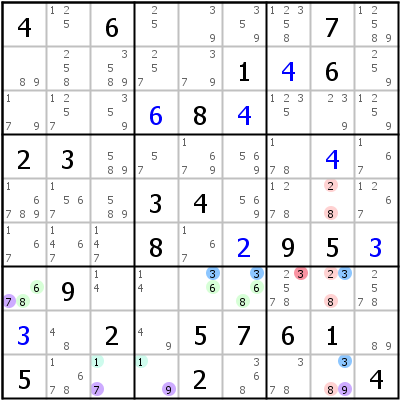
\includegraphics{./img/ALS_XY_Wing.png}
\caption{ALS XY Wing}
\end{center}
\end{figure}

\noindent Im oben stehenden Beispiel \textbf{Abbildung 4.19}\footnote{Beispiel aus \cite{HDKALSXYWing}} sieht man einen \textit{ALS XY Wing}, \textit{ALS} A ist hier Zeile 7 Spalten 1, 5 und 6 mit den Kandidaten 3, 6, 7 und 8, \textit{ALS} B ist Spalte 8 Zeilen 5, 7 und 9 mit den Kandidaten 2, 3, 8 und 9. \textit{ALS} C befindet sich in Zeile 9 Spalten 3 und 4 mit den Kandidaten 1, 7 und 9. x ist also 7, y ist 9 und z ist 3. Da z wegen der oben genannten Begründung nur in \textit{ALS} A und B vorkommen kann, können jetzt alle Kandidaten von z gelöscht werden, die von allen Instanzen von z in A und B gesehen werden. Das ist die Ziffer 3 in z7s7.